\subsection{The Perceptron} \label{sec:background-artificial-neural-networks-perceptron}

\begin{figure}[t]
	\centering
	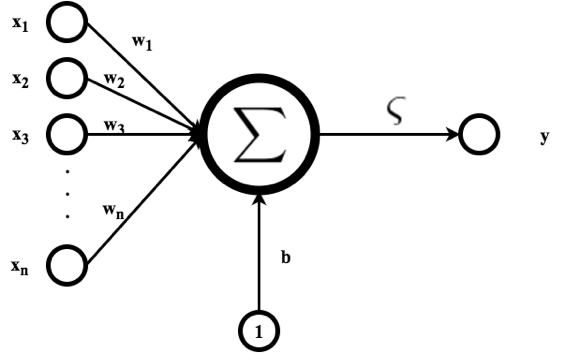
\includegraphics[max width=\textwidth]{perceptron}
	\caption{Visual depiction of a single artificial neuron, sometimes called a perceptron.}
	\label{fig:perceptron}
\end{figure}

Consider the problem of classifying a set of data points into one of several classes. We can reduce this problem to that of finding a decision function $\hat{f}(\vec{x})$ that approximates a true function $f(\vec{x})$, that maps a data point $\vec{x}$ to a class $\vec{y}$. The function $f(\vec{x})$ can be represented as a linear combination of the parameters of $\vec{x}$:
\begin{gather*}
	w_1 x_1 + w_2 x_2 + ... + w_n x_n + b = y_1\\
	w_1 x_1 + w_2 x_2 + ... + w_n x_n + b = y_2\\
	\vdots\\ 
	w_1 x_1 + w_2 x_2 + ... + w_n x_n + b = y_m
\end{gather*}
The problem of learning the decision function then becomes finding a set of weights ($w_1$ to $w_n$ and $b$) that satisfy the provided data points as well as generalize to yet unseen observations\cite{Le15atutorial}.

This system of equations can be depicted as a neuron, like that shown in Figure \ref{fig:perceptron}, that accepts weighted inputs and fires an output that is modified by an activation function. The weights in an artificial neuron resemble synaptic weights found in the neural networks of living organisms. Synaptic weights determine how much influence one neuron has on the next in the network. When considered in the context of artificial neural networks, the weights determine how much the corresponding part of the input affects the output and therefore they act as the medium by which the network is able to represent the decision function\cite{Mitchell}.  

The activation function on the other hand resembles the threshold potential of a natural neural network. It determines how the signal propagates through the system. Likewise, the activation functions of artificial neural networks determine the shape of the output of each unit. Figure \ref{fig:perceptron} shows a neuron with a sigmoid activation. The sigmoid activation function normalizes the output of the unit to a value between zero and one and also produces a non-linear output which is important for some functions\cite{Goodfellow-et-al-2016}.

Once fully trained, the neuron (also called a perceptron) is then used to predict the output of unseen observations using the following formulas:
\begin{gather}
\label{eq:sigmoid}
	z = b + \sum\limits_{i=1}^n x_i w_i\\
	y = \frac{1}{1+e^{-z}}
\end{gather}

\subsubsection{Gradient Descent Algorithm}

The process of discovering the optimum set of weights is performed using the gradient descent algorithm. Gradient descent involves updating the weights of the model in such a way as to minimize the error produced by  applying the training examples to the perceptron relative to the expected target output. The error is depicted as a cost function whose gradient we need to traverse in the negative direction to minimize the error. See Figure \ref{fig:gradient-descent}\cite{Le15atutorial}. The mean square error (MSE) is a popular cost function\cite{Mitchell} given by:
\begin{equation}
E(\vec{w}) = \frac{1}{2} \sum_{d \in D} (t_d - y_d)^2
\end{equation}
where $\vec{w}$ is a vector that comprises the neuron's weights, $D$ is the set of training examples, $t_d$ is the target output for the training example $d$ and $y_d$ is the actual output of the perceptron for training example $d$. 

Figure \ref{fig:gradient-descent} visualizes the error function. Initially the weights are set to random values that place the error at an undesirable level. By iteratively updating the weights, the error is reduced and the weights evolve to capture the decision function. The weight update rule for a linear perceptron where:
\begin{equation}
	y = b + \sum\limits_{i=1}^n x_i w_i\\
\end{equation}
is given by:
\begin{equation}
w_i \leftarrow w_i + \Delta w_i
\end{equation}
where
\begin{equation}
\Delta w_i = -\eta \frac{\partial E}{\partial w_i}
\end{equation}
$\eta$ is the learning rate. The learning rate is a positive value that determines the step size that the gradient descent will take. The larger the learning rate the quicker the descent, however this risks skipping over the optimal weights.

The change $\Delta w_i$ can be obtained by partially differentiating the error with respect to $w_i$:
\begin{equation}
\begin{split}
\frac{\partial E}{\partial w_i} & = \frac{\partial}{\partial w_i} \frac{1}{2} \sum_{d \in D} (t_d - y_d)^2\\
& = \frac{1}{2} \sum_{d \in D} \frac{\partial}{\partial w_i} (t_d - y_d)^2\\
& = \frac{1}{2} \sum_{d \in D} 2(t_d - y_d) \frac{\partial}{\partial w_i} (t_d - y_d) \\
& = \sum_{d \in D} (t_d - y_d) \frac{\partial}{\partial w_i} (t_d - \vec{w}.\vec{x_d}) \\
& = \sum_{d \in D} (t_d - y_d) (-x_{id})
\end{split}
\end{equation}
where $x_{id}$ is the input of training example $d$. The update rule is therefore given by:
\begin{equation} \label{eq:weight-update}
\Delta w_i = \eta \sum_{d \in D} (t_d - y_d) (x_{id})
\end{equation}

\begin{figure}[t]
	\centering
	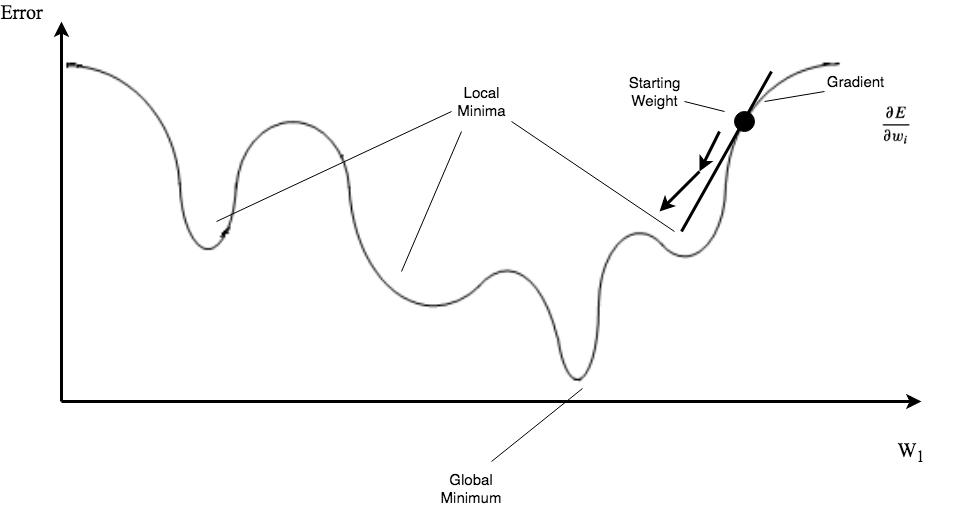
\includegraphics[max width=\textwidth]{gradient-descent}
	\caption{Weights are updated to minimize the error produced by the cost function in an effort to reach the global minimum.}
	\label{fig:gradient-descent}
\end{figure}

\subsubsection{Stochastic Approximation and Batch SGD}

Gradient descent can be considered a strategy for searching through a hypothesis space provided that the error can be differentiated with respect to the hypothesis parameters like the weights of a perceptron. There are two drawbacks however. First, gradient descent tends to be slow in converging on to a local minimum. Second, in more complex hypothesis spaces where there are many local minima, there is no guarantee that the gradient decent will reach the global minimum. There are two ways we can modify the gradient descent algorithm to optimize the learning process: stochastic approximation and batch stochastic gradient descent\cite{Mitchell}.

Instead of running all training examples through the gradient descent algorithm before summing up the error and calculating the weight update, with stochastic gradient descent we calculate the error and perform the weight updates after each training example is introduced to the network. Equation \ref{eq:weight-update} will therefore be replaced by:
\begin{equation}
\Delta w_i = \eta (t_d - y_d) (x_{id})
\end{equation}
This approach can take longer to train a network but has the advantage of adding a stochastic component due to the individual weight changes made for each example. This can increase the likelihood that the algorithm moves out of a local minimum and converges to a more optimal set of weights.\cite{Mitchell}.

A slight modification to the stochastic gradient descent (SGD) approach is to use batch SGD. With batch SGD, instead of updating the weights after every training example, the weights are updated after a batch of examples are introduced to the network. The batch size can vary and can have a significant impact on the training outcome. Using batches of examples maintains some of the speed up of the original gradient descent approach while also retaining the stochastic weight changes that can lead to better models. Batch SGD is used extensively in the experiments presented in Chapter 4.

\subsubsection{Adam Optimizer}

The learning rate is an important hyper parameter that can speed up the learning process when increased. However, higher learning rates can prevent the gradient descent algorithm from reaching a desired minimum in the hypothesis space, especially when the current gradient is close to that desired minimum. One modification that can be made is to introduce a learning rate decay parameter. With learning rate decay, after every epoch (a single iteration where all training examples are introduced to the network) the learning rate is decreased by a factor defined by the decay rate. This makes training faster early in the gradient descent where it is highly unlikely the algorithm will skip a desired minimum and prevents this from happening the closer we converge onto a minimum\cite{Mitchell}.

Other gradient descent techniques introduce a momentum factor to achieve the same goal. This momentum factor prevents the descent algorithm from changing direction too fast. This allows the algorithm to skip smaller shallow local minimums and also to continue down the slope faster when there is no change in gradient\cite{Mitchell}.

Some gradient descent techniques that have grown in popularity over the past decade take learning rate adaptation a step further. The Adam optimizer is one such algorithm that is an extension of the stochastic gradient descent. With Adam optimizer, every weight in the model has its own learning rate. This allows the algorithm to find a solution in a hypothesis space with sparse gradients (where the majority of weights are zero) such as those exhibited by computer vision problems\cite{DBLP:journals/corr/KingmaB14}.

Adam also uses moment to adapt each learning rate based on the current gradient of the parameter in question. Like momentum based techniques, moment allows the algorithm to go down the slope faster when there is little change in the gradient. However, this is done by adapting the learning rate instead of adding an additional factor. Specifically, Adam calculates an exponential moving average for the gradient and the square of the gradient. The learning rate is changed based on these averages and beta1 and beta2 values given as parameters to the optimizer\cite{DBLP:journals/corr/KingmaB14}.  Adam optimizer uses the following parameters with the following recommended values:
\begin{itemize}
	\item Alpha is the initial learning rate and is set to $0.001$
	\item Beta1 the rate by which the exponential moving average is decayed and is set to $0.9$
	\item Beta2 is the rate by which the exponential moving average  of the square of the gradient is decayed and is set to $0.999$
	\item Epsilon is a factor that prevents division by zero  and is usually set to $10^{-8}$
\end{itemize}	

The Adam optimizer is more efficient than other techniques that use a separate learning rate for each parameter. It also allows converging to a solution in the hypothesis space much faster than typical stochastic gradient descent\cite{DBLP:journals/corr/KingmaB14}. For these two reasons, the experiments conducted as part of the research presented in this thesis use the Adam optimizer exclusively as implemented in the TensorFlow library.
